This test problem is for a homogeneous absorber medium with an incident
flux, which has a simple exponential decay solution.
The problem summary is given in Table \ref{tab:absorber}.

%-------------------------------------------------------------------------------
\begin{table}[htb]\caption{Convergence Test Problem 2 Summary}
\label{tab:absorber}
\centering
\begin{tabular}{l l}\toprule
\emph{Parameter} & \emph{Value}\\\midrule
Domain & $\mathcal{D} = (0,1)$\\
Boundary Conditions & $\scalarsolution(x)=1,\quad x\in\partial\mathcal{D}^-$,\\
   & $\quad\partial\mathcal{D}^-=\{x\in\partial\mathcal{D}:\mathbf{n}(x)
       \cdot\mathbf{\Omega}<0\}$\\
Direction & $\mathbf{\Omega} = \mathbf{e}_x$\\
Cross Section & $\reactioncoef(x)=10$\\
Source & $\scalarsource(x)=0$\\
Speed & $\speed=1$\\
Exact Solution & $\scalarsolution(x)=e^{-10x}$\\
\bottomrule\end{tabular}
\end{table}
%-------------------------------------------------------------------------------

This problem was run in steady-state to avoid temporal error so that spatial
convergence rates could accurately be measured.
The coarsest mesh size in this study uses 8 cells, and each successive mesh
size is halved, with the finest mesh in the study using 256 cells.
The run parameters for this test problem are given in Table
\ref{tab:absorber_ss_run_parameters}.

%-------------------------------------------------------------------------------
\begin{table}[htb]
\caption{Convergence Test Problem 2 Run Parameters}
\label{tab:absorber_ss_run_parameters}
\centering
\begin{tabular}{l l}\toprule
\emph{Parameter} & \emph{Value}\\\midrule
Number of Cells & $N_{cell} = 8,16,\mathbf{32},64,128,256$\\
Time Discretization & Steady-State\\
Boundary Conditions & Strong Dirichlet with
  $\limiterletter_i^-=\limiterletter_i^+=1$\\\midrule
Entropy Function & $\entropy(\scalarsolution) = \frac{1}{2}\scalarsolution^2$\\
Entropy Residual Coefficient & $\entropyresidualcoef = 0.1$\\
Entropy Jump Coefficient & $\entropyjumpcoef = 0.1$\\\midrule
FCT Solution Bounds & Analytic\\
FCT Initial Guess & $\scalarsolution^{(0)} = \scalarsolution^H$\\
\bottomrule\end{tabular}
\end{table}
%-------------------------------------------------------------------------------

Figure \ref{fig:absorber_ss_solution} shows a comparison of the solutions with
32 cells, and Figure \ref{fig:absorber_ss_visc} shows the corresponding
viscosity profiles.
The FCT methods use the analytic solution bounds
given by Equation \eqref{eq:analyticDMP_ss}.

%-------------------------------------------------------------------------------
\begin{figure}[ht]
   \centering
      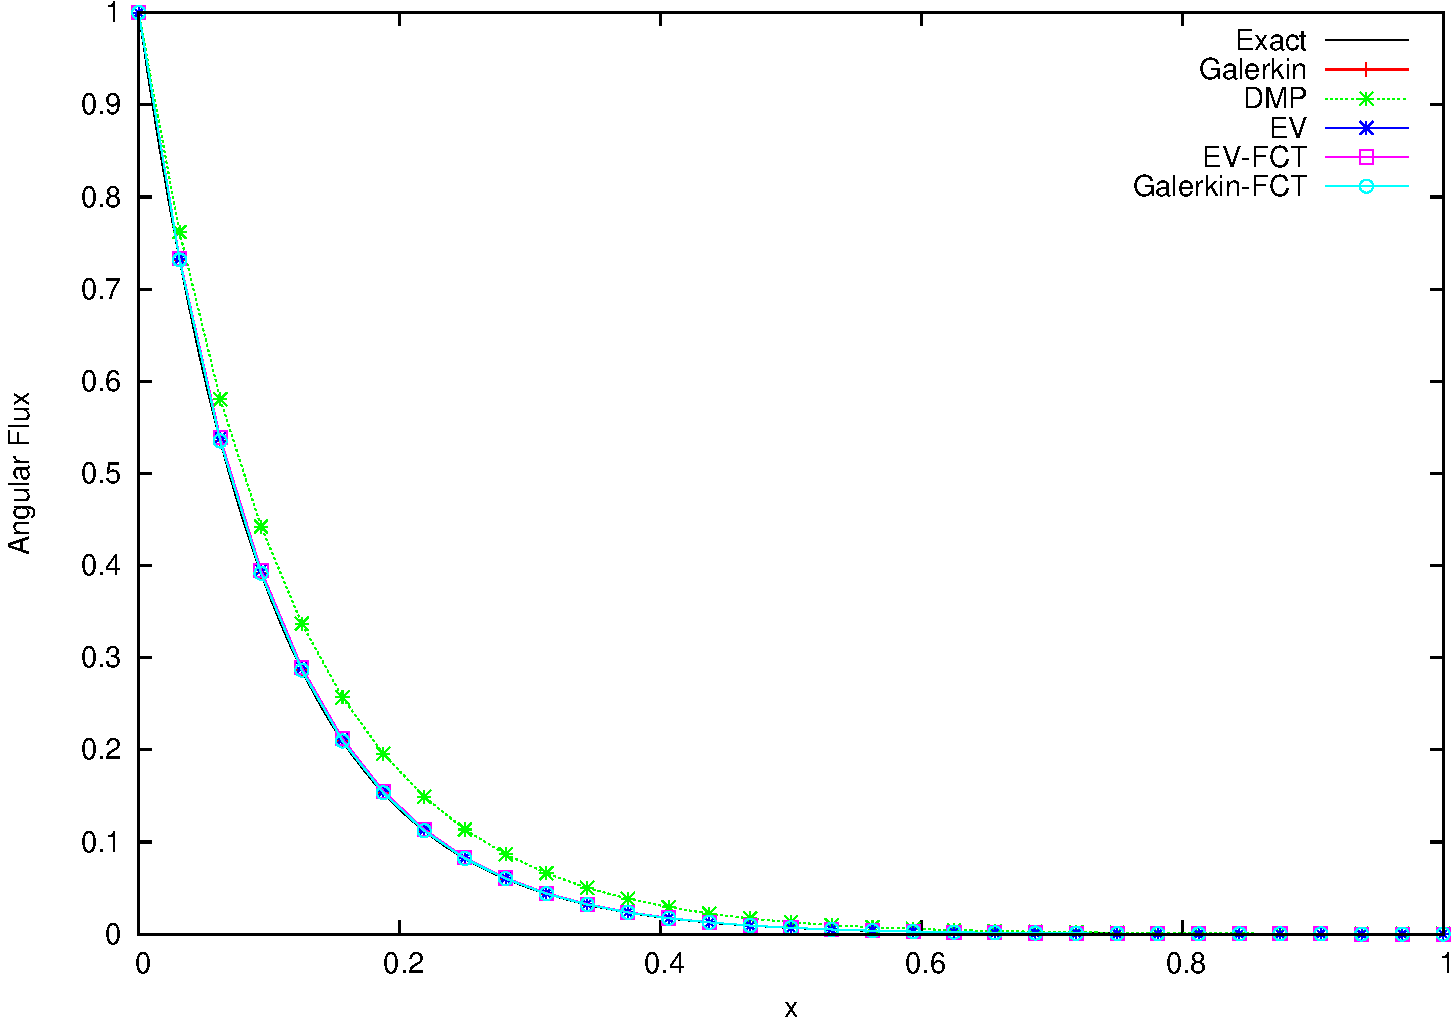
\includegraphics[width=\textwidth]
        {\contentdir/results/transport/absorber_ss/images/angularflux_SS.pdf}
      \caption{Comparison of Solutions for Convergence Test Problem 2 with 32 Cells}
   \label{fig:absorber_ss_solution}
\end{figure}
%-------------------------------------------------------------------------------
%-------------------------------------------------------------------------------
\begin{figure}[ht]
   \centering
      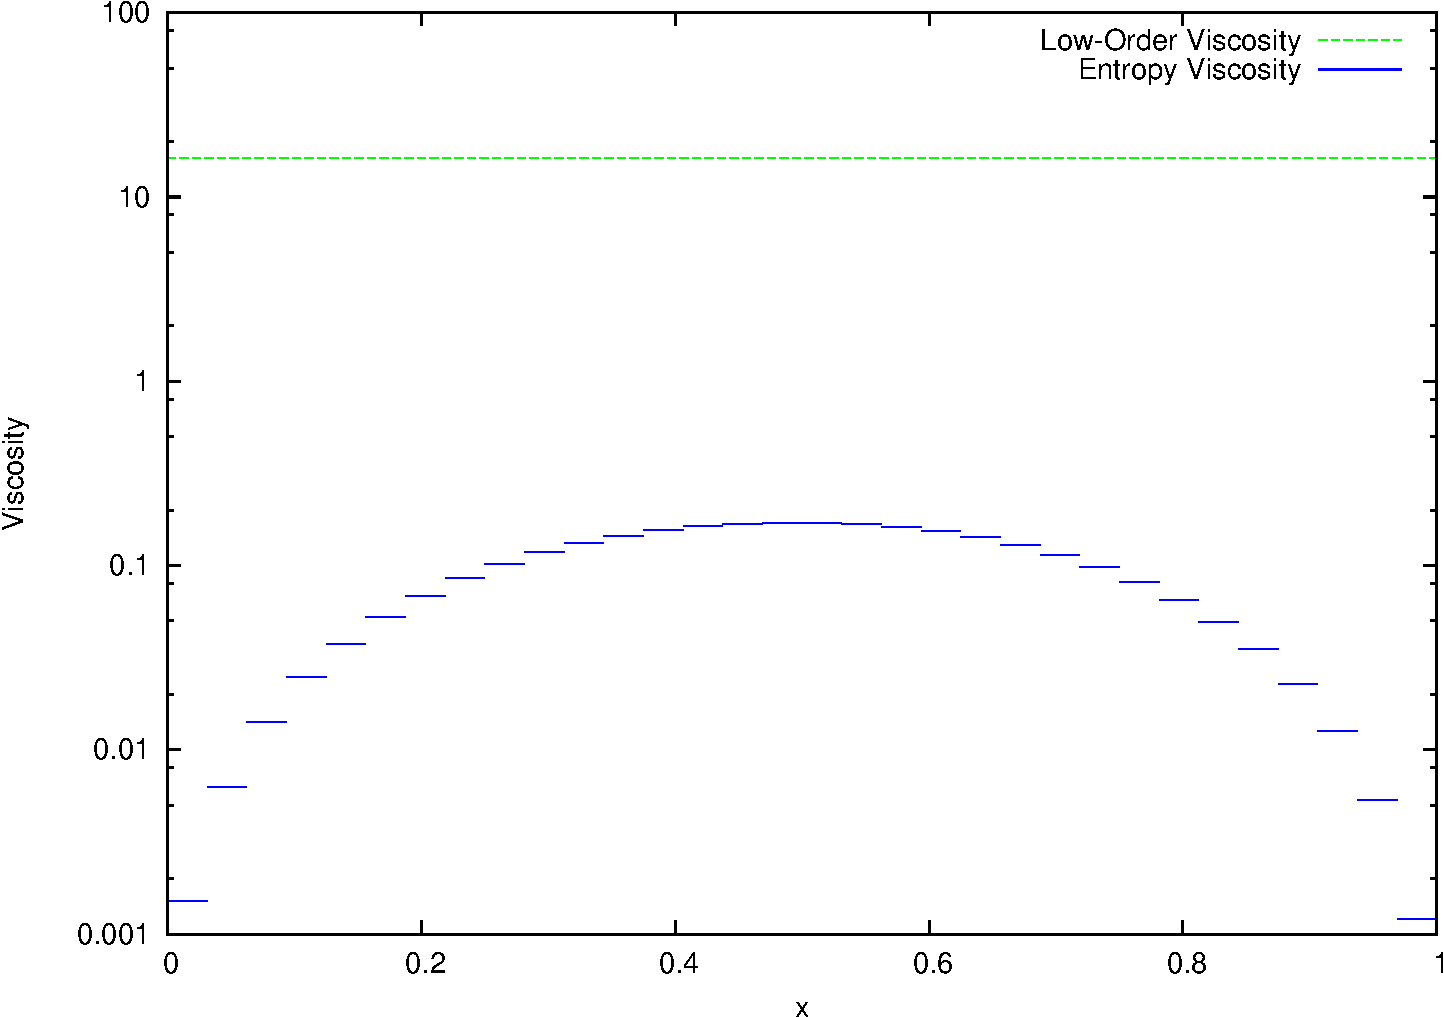
\includegraphics[width=\textwidth]
        {\contentdir/results/transport/absorber_ss/images/viscosity_SS.pdf}
      \caption{Viscosity Profiles for Convergence Test Problem 2 with 32 Cells}
   \label{fig:absorber_ss_visc}
\end{figure}
%-------------------------------------------------------------------------------

Figure \ref{fig:absorber_ss_convergence} shows a comparison of
errors with different methods. The DMP low-order method achieves first-order
spatial convergence as expected, and the Galerkin and Galerkin-FCT methods achieve
second-order accuracy. The entropy viscosity and entropy-viscosity-FCT
(EV-FCT) methods start out with more error than the Galerkin methods
in the coarse meshes, but converge with order greater than 2 until
the finer meshes, where the convergence of the EV methods 
asymptotically approach that of the Galerkin methods.

%-------------------------------------------------------------------------------
\begin{figure}[ht]
   \centering
      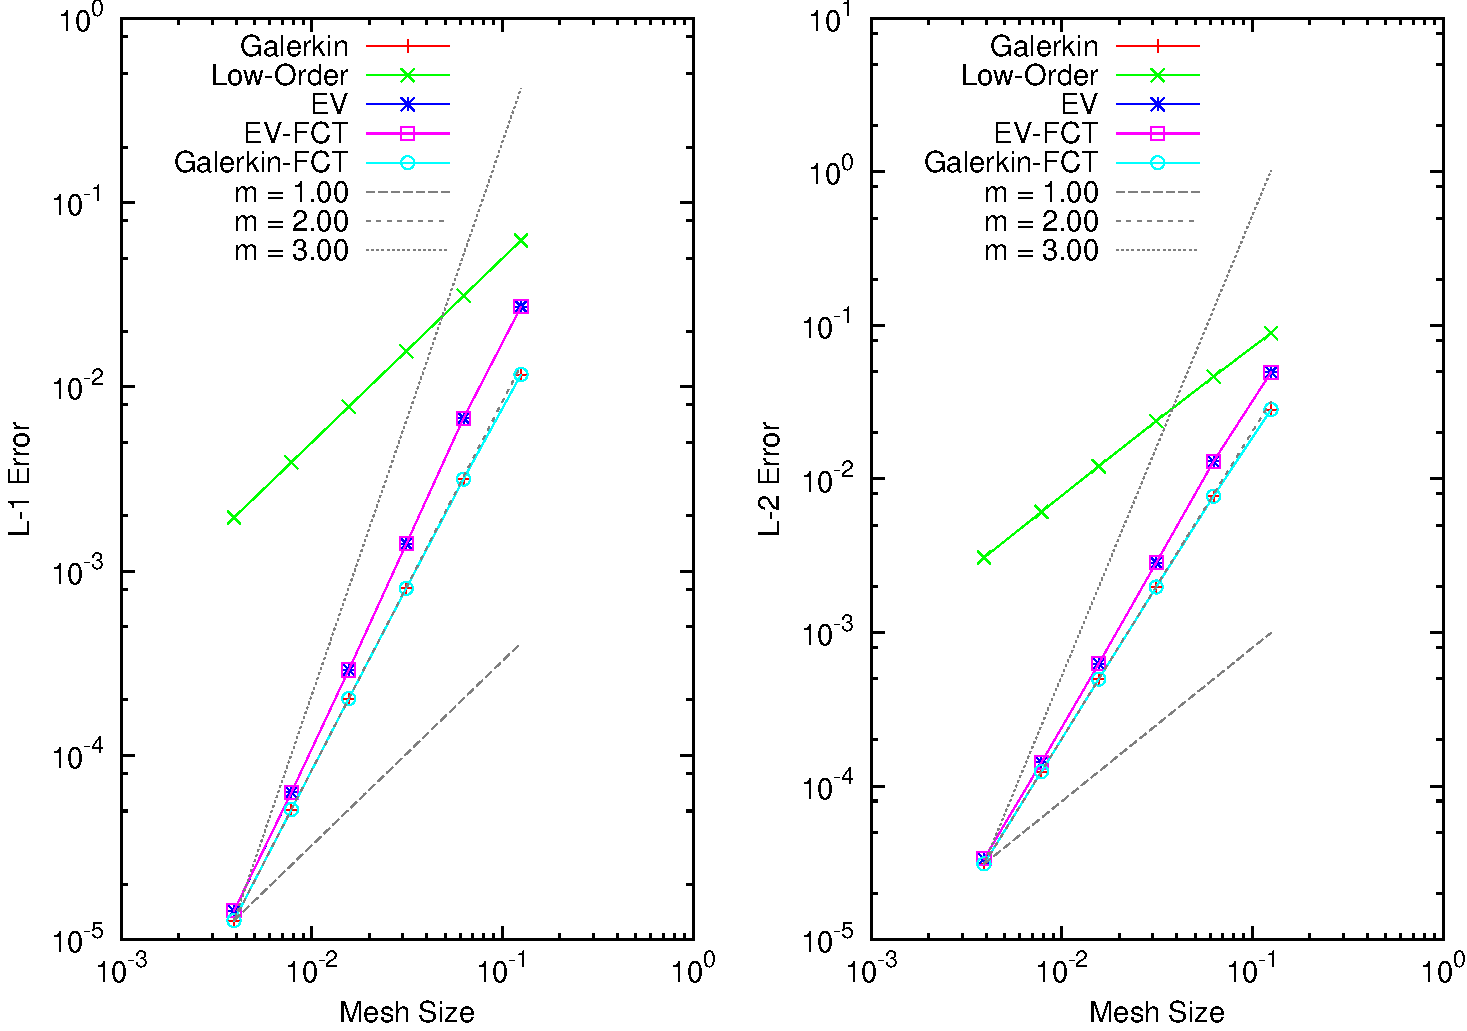
\includegraphics[width=\textwidth]
        {\contentdir/results/transport/absorber_ss/images/convergence_SS.pdf}
      \caption{Comparison of Errors for Convergence Test Problem 2}
   \label{fig:absorber_ss_convergence}
\end{figure}
%-------------------------------------------------------------------------------

Figure \ref{fig:absorber_ss_entropy_convergence} shows the convergence of the
$L^2$ norm entropy residual $\entropyresidual$ and entropy jumps $\entropyjump$,
which are computed as
\begin{equation}
  \|\entropyresidual\|_{L^2(\domain)} = \sqrt{\int\limits_\domain
    \entropyresidual(\x)^2\dvolume
  } \eqc
\end{equation}
\begin{equation}
  \|\entropyjump\|_{L^2(\domain)} = \sqrt{\int\limits_\domain
    \entropyjump(\x)^2\dvolume
  } = 
  \sqrt{\sum_\cell \entropyjump_\cell^2\cellvolume} 
  \eqc
\end{equation}
where $\entropyjump(\x)$ is the piecewise constant function such that
$\entropyjump(\x)=\entropyjump_\cell$ for $\x\in\celldomain$.
For this study, the coarsest mesh consists of 2 cells, and there are a total of
12 refinement levels, so the final refinement level corresponds to
$2^12$ cells. The entropy residual $L^2$ norm converges first-order
as expected. The entropy jumps $L^2$ norm actually increases for the coarsest
meshes, until meshes finer than roughly 32 cells, where it transitions
to first-order convergence.

%-------------------------------------------------------------------------------
\begin{figure}[ht]
   \centering
      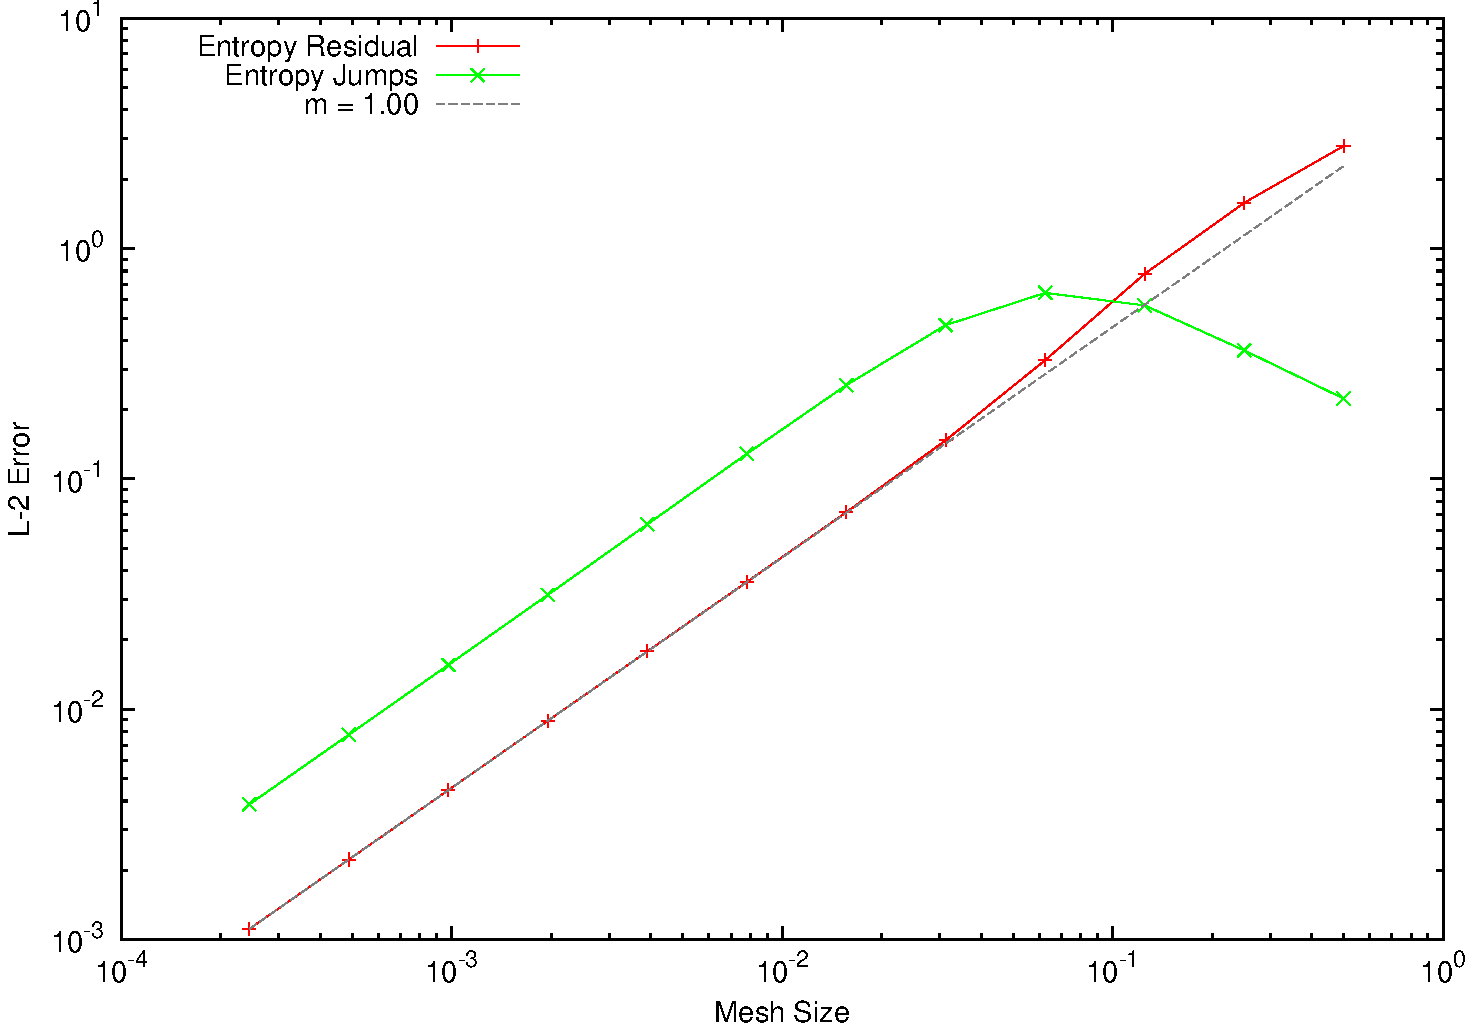
\includegraphics[width=\textwidth]
        {\contentdir/results/transport/absorber_ss/images/entropy_convergence.pdf}
      \caption{Convergence of Entropy Residual and Entropy Jumps for
        Convergence Test Problem 2}
   \label{fig:absorber_ss_entropy_convergence}
\end{figure}
%-------------------------------------------------------------------------------

\clearpage
